\documentclass[a4paper,12pt]{article}
\usepackage[a4paper, top=3cm, bottom=3cm, left=3cm, right=3cm]{geometry}

\usepackage{float}

\usepackage[style=alphabetic,sorting=nyt]{biblatex}
% setting the path to the bib file
\addbibresource{sources.bib}

\usepackage{amsfonts}
\usepackage{amsmath}
\usepackage{amssymb}

\usepackage{graphicx}
\usepackage{xcolor}

\usepackage{pdfpages}
\usepackage{tocloft}
\setcounter{tocdepth}{3}

\usepackage{tikz}
\usepackage{pgfplots}

\usepackage{hyperref}
\hypersetup{
  colorlinks=false,
  linkcolor=blue,
  filecolor=magenta,
  urlcolor=blue,
}
\usepackage[english]{babel}
\usepackage{lastpage}
\usepackage{fancyhdr}
\pagestyle{fancy}
\fancyhf{}
\renewcommand{\headrulewidth}{0pt}
\rfoot{Page \thepage\ of \pageref{LastPage}}

\setlength{\parskip}{1em}
\setlength{\parindent}{0px}

\title{A unifying framework for quanitifying the data propogation bottlenecks of graph representation learning methods}

\author{
  \color{red}  Mustafa Hekmat Al-Abdelamir\\
  \color{red}  Joshua Victor Niemelä\\
}
\date{\today}


\begin{document}


\maketitle



\section{Introduction}

Topological Deep Learning (TDL) is gaining traction as a novel approach~\cite{papamarkou_position:_2024} for Graph Representation Learning (GRL).
Leveraging topology, TDL has shown promising results in alleviating various limitations of Graph Neural Networks (GNNs)~\cite{horn_topological_2022}.

Two often-cited related\cite{giraldo_trade-off_2023} shortcomings in GNNs are over-smoothing and over-squashing.
Over-smoothing occurs when individual node features become washed out and too similar after multiple graph convolutions~\cite{li_deeper_2018}.
In message-passing, nodes send fixed-size messages to their neighbours, said neighbours aggregate the messages, update their features, then send out new messages and so on.
This process inevitably leads to information loss, as an increasingly large amount of information is compressed into fixed-size vectors.
This is known as over-smoothing~\cite{alon_bottleneck_2021}.

Still, perhaps because of the young nature of the field, there is limited theoretical foundation for quantifying these possible advantages.
This poses a problem in making quantitative comparisons between various architectures for GRL.
In this paper, we attempt to lay the foundations for various metrics to provide insights on over-squashing and over-smoothing and how they relate to the model's ability to learn.
To verify and support our theoretical foundations, we also run benchmarks against other approaches used for learning on graph data~\cite{horn_topological_2022}

\section{Data}
We will be using the QM9 dataset~\cite{blum}\cite{rupp} as real-world data to benchmark our models against
other models from the cited papers and to test the metrics we will develop.

We will also be creating and using synthetic datasets as this will give us more control over the data and allow us to create specific topological features and properties that we can then use to test the metrics and models.

\section{Methods}
\begin{itemize}
	\item  We will be using PyTorch Geometric to build our models and to replicate models cited in other papers as a comparison and empirical exploration of GRL.
	\item Docker will be used to containerise our experiments and replications to ensure reproducibility as well as make it easier to run experiments on different machines.
\end{itemize}

\section{Learning Objectives}


\begin{enumerate}
	\item Gain a solid understanding of the theoretical foundations of GNNs.
	\item Investigate the over-squashing problem in GNNs and how it affects the ability of the model to learn long-range dependencies~\cite{alon_bottleneck_2021}.
	\item Gain insights and understanding about TDL, how topology is leveraged for learning, and how it relates to the aforementioned bottlenecks~\cite{horn_topological_2022}.
	\item Construct generalisable metrics to quantify various geometric and topological properties of GNNs and the datasets they are trained on.
	\item Construct a model, for instance, a transformer or CCNN~\cite{tdlbook}, that can learn topological features in data and benchmark against non-topological approaches.
\end{enumerate}


\section{Three-node GCN}

To dip our toes into Graph Neural Netowrks and eventually the over-squashing problem,
we started out with a simple GCN model with one layer and one input channel (each node has only one feature).
Since the GCN aggregates all node connections, including self-connections with the same coeffecient, the GCN layer has exactly one parameter.
The update and aggregate function with normalisation enabled is described in eq \ref{GCN_AGG_W_NORM}. The trainable parameter is \(\Theta\).
\begin{equation}
  \mathbf{x}_i' = \Theta \sum_{j \in \mathcal{N}(v) \cup \{i\}} \frac{e_{j,i}}{\sqrt{\hat{d}_j \hat{d}_i}} \mathbf{x}_j
  \label{GCN_AGG_W_NORM}
\end{equation}

The formula without normalisation in \ref{GCN_AGG} is identical, albeit without the diagonal degree matrix term.
\begin{equation} \label{GCN_AGG}
  \mathbf{x}_i' = \Theta \sum_{j \in \mathcal{N}(v) \cup \{i\}} e_{j,i} \mathbf{x}_j
\end{equation}

Our dataset / problem is a graph of three nodes, with two children pointing into the root node. The root node is set to 0 (\(x_{1}=0\)) and the children have some random integer, the target is the sum of the entire graph. The readout is only done by reading the root node values.
\begin{figure}[H]
  \centering
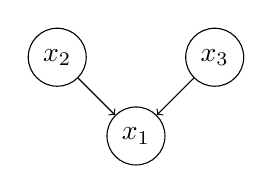
\begin{tikzpicture}
  % Define the nodes
  \node[circle, draw] (0) at (0, 0) {$x_{1}$};
  \node[circle, draw] (1) at (-1, 1) {$x_2$};
  \node[circle, draw] (2) at (1, 1) {$x_3$};

  % Draw the arrows
  \draw[->] (1) -- (0);
  \draw[->] (2) -- (0);
\end{tikzpicture}
\label{fig:three_node_graph}
\caption{The three-node graph}
\end{figure}

Algebraically, this problem is solved by
\begin{equation}
x_{1}' = x_{2}+x_{3} \label{three_node_solution}
\end{equation}


We first compute what the learnable parameter should be with, and without normalisation, and then we try to train the model and verify that we get the expected weights. The motivation behind this is to construct the simplest possible GNN problem and to solve it both by hand and computationally to understand how the GCN model works and how it learns.

Our edge weights are fixed to 1, which means all edges have equal weighting, \(e_{j, i}=1\) in eq \ref{GCN_AGG}. Since we only do one graph convolution towards the root, we can disregard the updates for the two children nodes and only look at the update that affects the root, which means we can set \(i=1\) as well in eq \ref{GCN_AGG}.

This leaves us with a linear function with one parameter as can be seen in eq \ref{three_node_solution}.
\begin{align} \label{three_node_solution}
  \mathbf{x}_1' &= \Theta \sum_{j \in \mathcal{N}(v) \cup \{1\}} \mathbf{x}_j,\ \Theta \in \mathbb{R}\\
   &= \Theta (x_{1} + x_{2} + x_{3}) \quad \text{note that } x_{1} = 0\\
                &= \Theta (x_{2} + x_{3}) \implies \Theta = 1
\end{align}

Next, we do the same for the normalised example, $\hat{d}_{i}$ is the number of neighbours of node $i$ plus one. This means, we have $\hat{d}_{2} = \hat{d}_{3} = 1$ and $\hat{d}_{1}=3$.
\begin{align}
  \mathbf{x}_1' &= \Theta \sum_{j \in \mathcal{N}(v) \cup \{i\}} \frac{1}{\sqrt{\hat{d}_j \hat{d}_i}} \mathbf{x}_j\\
  &= \Theta  \left( \frac{1}{\sqrt{\hat{d}_2 \hat{d}_1}} \mathbf{x}_2 +  \frac{1}{\sqrt{\hat{d}_3 \hat{d}_1}} \mathbf{x}_3 \right)\\
  &= \Theta  \left( \frac{1}{\sqrt{1 \cdot 3}} \mathbf{x}_2 +  \frac{1}{\sqrt{1 \cdot 3}} \mathbf{x}_3 \right)\\
  &= \frac{\Theta}{\sqrt{3}}  \left(  \mathbf{x}_2 +   \mathbf{x}_3 \right) \implies \theta = \sqrt{3} \approx 1.732\\
\end{align}

SHOW RESULTS HERE (
Homework for Mustafa)

Next, we tried a classification problem, which also turned out to be slightly more complex. We reused the same graph. But this time we want to classify if $x_{1} = x_{2}+x_{3}$ is true or not for the given graph. \(x_2, x_3\) are integers sampled from a uniform distribution in the range \([0, 10[\). Half of the generated graphs will have the property that \(x_{1} = x_{2}+x_{3}\) and the other half \(x_1\) is a random integer in the range \([0, 20[\).

We tried with the same GCN model, here we got an accuracy of 48.5\%. Since this is close to the actual distribution of the classe, we can conclude that the model has not the objective function.

The motivation of our following experiments is that we want the aggregator to find the difference between the children nodes and the root node. Hence we want to add the neighbours to the root but subtract the root node itself. Hence the self loop needs a separate weight parameter.

Hence we tried using a SAGE model, this is the same as the GCN model but with
an additional weight parameter for the self-loop, we also gave it a bias parameter. We got an accuracy of 53\%. % aber why do we give it a bias parameter?
This is not much better than the GCN model.

The models fail to learn since we have no non-linearity in the model. We need some behaviour
that allows the model to learn that the further away from 0 the difference is,
the more likely it is that the children nodes don't sum to the root node.
Therefore, we want a function that maps 0 to 1 and values further away from 0 to 0. 
For this, we simply chose the gaussian function \(e^{-x^2}\) which we
appended to the readout of the model. With this we get perfect results with an
accuracy of 100\%.





\section{Tree neighbours-match}
We decided to try to reproduce the over-squashing problem from \cite{alon_bottleneck_2021}.
\subsection{Data}
The dataset of a given depth $d$ is comprised of binary trees of depth $d$ and $n$ unique iid. trees. Each node of the graph has two features, a class, and the number of ``leaves''. We can represent a tree as a directed and connected graph $G \in (V, E)$ where $(i, j) \in E$ [COMMENT FROM RAGHAV?].
We let $A$ represent the adjacency matrix for a given tree without any self-loops. Let $A_{i,j}= \text{if } \lfloor \frac{i}{2}\rfloor = j \text{ then } 1 \text{ else } 0$. We use self-loops since they have a positive effect on performance [CITE THE CURVATURE PAPER(?)]: $\bar{A}=A+I$, where $I$ is the identity matrix.

The $V \in \mathbb{N}^{2 \times n}$ contain our attributes for the nodes. All nodes other than nodes at depth $d$ have a class of 0: $V_{1, i_{1}} = 0, i_{1} \in \{0, 1, 2, \ldots, n-2^{d}-1, n-2^{d}\}$. The remaining nodes are labelled in ascending order: $V_{1, i_{2}}= i_{2}-(n-2^{d}), i_{2} \in \{n-2^{d}+1, \ldots, n-1, n\}$.
The root has a random number of leaves between $1$ and $2^{d}$. The nodes in the last layer are sampled to have a random number of leaves between $1$ and $2^{d}$ without replacement. All nodes between depth $1$ to $d-1$ are set to have 0 leaves. The label for the dataset is then finally set to be the class whose leaves match the number of leaves of the root. Note that the edge matrix is 1-indexed and the attribute matrix is 0-indexed for ease of notation.

NOTE:
Our tree neighbours using the approximation fr birthday problem has almost 0 likelihood for collisions between test and train


\section{NOTES FROM RESEARCH THAT HAVE NOT BEEN ORGANISED!}

For each given depth $d$, we have $2^{d}! \cdot 2^{d}$ ($2^{d}!$ permutations of the bottom layer, $2^{d}$ possible root labels) possible trees / samples. We notice this means that for $d=2$ and $d=3$, we only get $96$ and $322560$ unique trees respectively.
We sample from this dataset by generating a binary tree, then creating a permutation of the unique number of leaves and then randomly picking a class that the root should mimic.

By the birthday paradox, we know this means these depths will very likely contain duplicate entries in the train and test data. Since they are both sampled IID this means it will not result in overfitting. In the event that the model has perfectly learnt the training data which contains all possible unique entries, we know that any future samples we throw at the model will also just contain the same entries we can classify.
For depths greater then 3, the number of unique trees grows to the point where the likelihood of duplicate entries goes towards 0.


\subsection{Running the experiment} % tree neighbours-match

Although in \cite{alon_bottleneck_2021}, the authors present their findings on the tree neighbours-match dataset, they do not provide results of implementing the fully adjacent last layer which they otherwise more widely propose as a heuristic approach to deal with over-squashing.
This has led us to implement the fully adjacent last layer and compare the model with and without the last layer. We have in total run 1135 experiments, with a random distribution of parameters, to see how the GCN models with and without the fully adjacent last layer compare. The results are presented in Figure \ref{fig:tree_experiment_graph}. More detailed results can be found \href{PLACE SOMETHING HERE MAYBE A LINK TO THE RESULTS IN THE}{here}.

\begin{figure}[H]
	\centering
	% Recommended preamble:
\usetikzlibrary{arrows.meta}
\usetikzlibrary{backgrounds}
\usepgfplotslibrary{patchplots}
\usepgfplotslibrary{fillbetween}
\pgfplotsset{%
    layers/standard/.define layer set={%
        background,axis background,axis grid,axis ticks,axis lines,axis tick labels,pre main,main,axis descriptions,axis foreground%
    }{
        grid style={/pgfplots/on layer=axis grid},%
        tick style={/pgfplots/on layer=axis ticks},%
        axis line style={/pgfplots/on layer=axis lines},%
        label style={/pgfplots/on layer=axis descriptions},%
        legend style={/pgfplots/on layer=axis descriptions},%
        title style={/pgfplots/on layer=axis descriptions},%
        colorbar style={/pgfplots/on layer=axis descriptions},%
        ticklabel style={/pgfplots/on layer=axis tick labels},%
        axis background@ style={/pgfplots/on layer=axis background},%
        3d box foreground style={/pgfplots/on layer=axis foreground},%
    },
}

\begin{tikzpicture}[/tikz/background rectangle/.style={fill={rgb,1:red,1.0;green,1.0;blue,1.0}, fill opacity={1.0}, draw opacity={1.0}}, show background rectangle]
\begin{axis}[point meta max={nan}, point meta min={nan}, legend cell align={left}, legend columns={1}, title={}, title style={at={{(0.5,1)}}, anchor={south}, font={{\fontsize{14 pt}{18.2 pt}\selectfont}}, color={rgb,1:red,0.0;green,0.0;blue,0.0}, draw opacity={1.0}, rotate={0.0}, align={center}}, legend style={color={rgb,1:red,0.0;green,0.0;blue,0.0}, draw opacity={1.0}, line width={1}, solid, fill={rgb,1:red,1.0;green,1.0;blue,1.0}, fill opacity={1.0}, text opacity={1.0}, font={{\fontsize{8 pt}{10.4 pt}\selectfont}}, text={rgb,1:red,0.0;green,0.0;blue,0.0}, cells={anchor={center}}, at={(0.98, 0.98)}, anchor={north east}}, axis background/.style={fill={rgb,1:red,1.0;green,1.0;blue,1.0}, opacity={1.0}}, anchor={north west}, xshift={1.0mm}, yshift={-1.0mm}, width={150.4mm}, height={99.6mm}, scaled x ticks={false}, xlabel={Tree depth}, x tick style={color={rgb,1:red,0.0;green,0.0;blue,0.0}, opacity={1.0}}, x tick label style={color={rgb,1:red,0.0;green,0.0;blue,0.0}, opacity={1.0}, rotate={0}}, xlabel style={at={(ticklabel cs:0.5)}, anchor=near ticklabel, at={{(ticklabel cs:0.5)}}, anchor={near ticklabel}, font={{\fontsize{11 pt}{14.3 pt}\selectfont}}, color={rgb,1:red,0.0;green,0.0;blue,0.0}, draw opacity={1.0}, rotate={0.0}}, xmajorgrids={true}, xmin={1.5072}, xmax={5.4928}, xticklabels={{$2$,$3$,$4$,$5$}}, xtick={{2.0,3.0,4.0,5.0}}, xtick align={inside}, xticklabel style={font={{\fontsize{8 pt}{10.4 pt}\selectfont}}, color={rgb,1:red,0.0;green,0.0;blue,0.0}, draw opacity={1.0}, rotate={0.0}}, x grid style={color={rgb,1:red,0.0;green,0.0;blue,0.0}, draw opacity={0.1}, line width={0.5}, solid}, axis x line*={left}, x axis line style={color={rgb,1:red,0.0;green,0.0;blue,0.0}, draw opacity={1.0}, line width={1}, solid}, scaled y ticks={false}, ylabel={Max train accuracy}, y tick style={color={rgb,1:red,0.0;green,0.0;blue,0.0}, opacity={1.0}}, y tick label style={color={rgb,1:red,0.0;green,0.0;blue,0.0}, opacity={1.0}, rotate={0}}, ylabel style={at={(ticklabel cs:0.5)}, anchor=near ticklabel, at={{(ticklabel cs:0.5)}}, anchor={near ticklabel}, font={{\fontsize{11 pt}{14.3 pt}\selectfont}}, color={rgb,1:red,0.0;green,0.0;blue,0.0}, draw opacity={1.0}, rotate={0.0}}, ymajorgrids={true}, ymin={0.044835937500000034}, ymax={1.0278203125}, yticklabels={{$0.1$,$0.2$,$0.3$,$0.4$,$0.5$,$0.6$,$0.7$,$0.8$,$0.9$,$1.0$}}, ytick={{0.1,0.2,0.3,0.4,0.5,0.6,0.7,0.8,0.9,1.0}}, ytick align={inside}, yticklabel style={font={{\fontsize{8 pt}{10.4 pt}\selectfont}}, color={rgb,1:red,0.0;green,0.0;blue,0.0}, draw opacity={1.0}, rotate={0.0}}, y grid style={color={rgb,1:red,0.0;green,0.0;blue,0.0}, draw opacity={0.1}, line width={0.5}, solid}, axis y line*={left}, y axis line style={color={rgb,1:red,0.0;green,0.0;blue,0.0}, draw opacity={1.0}, line width={1}, solid}, colorbar={false}]
    \addplot[color={rgb,1:red,0.0;green,0.0;blue,0.0}, name path={13}, area legend, fill={rgb,1:red,0.0;green,0.6056;blue,0.9787}, fill opacity={1.0}, draw opacity={1.0}, line width={1}, solid]
        table[row sep={\\}]
        {
            \\
            1.8  1.0  \\
            1.71  1.0  \\
            1.8900000000000001  1.0  \\
            1.8  1.0  \\
            1.8  1.0  \\
        }
        ;
    \addlegendentry {base}
    \addplot[color={rgb,1:red,0.0;green,0.0;blue,0.0}, name path={13}, area legend, fill={rgb,1:red,0.0;green,0.6056;blue,0.9787}, fill opacity={1.0}, draw opacity={1.0}, line width={1}, solid, forget plot]
        table[row sep={\\}]
        {
            \\
            1.98  1.0  \\
            1.98  1.0  \\
            1.62  1.0  \\
            1.62  1.0  \\
            1.98  1.0  \\
            1.98  1.0  \\
        }
        ;
    \addplot[color={rgb,1:red,0.0;green,0.0;blue,0.0}, name path={13}, area legend, fill={rgb,1:red,0.0;green,0.6056;blue,0.9787}, fill opacity={1.0}, draw opacity={1.0}, line width={1}, solid, forget plot]
        table[row sep={\\}]
        {
            \\
            1.98  1.0  \\
            1.62  1.0  \\
            1.62  1.0  \\
            1.98  1.0  \\
            1.98  1.0  \\
            1.8  1.0  \\
        }
        ;
    \addplot[color={rgb,1:red,0.0;green,0.0;blue,0.0}, name path={13}, area legend, fill={rgb,1:red,0.0;green,0.6056;blue,0.9787}, fill opacity={1.0}, draw opacity={1.0}, line width={1}, solid, forget plot]
        table[row sep={\\}]
        {
            \\
            1.8  1.0  \\
            1.71  1.0  \\
            1.8900000000000001  1.0  \\
            1.8  1.0  \\
            1.8  1.0  \\
        }
        ;
    \addplot[color={rgb,1:red,0.0;green,0.0;blue,0.0}, name path={13}, area legend, fill={rgb,1:red,0.0;green,0.6056;blue,0.9787}, fill opacity={1.0}, draw opacity={1.0}, line width={1}, solid, forget plot]
        table[row sep={\\}]
        {
            \\
            2.8  0.96340625  \\
            2.71  0.96340625  \\
            2.8899999999999997  0.96340625  \\
            2.8  0.96340625  \\
            2.8  0.9828281249999999  \\
        }
        ;
    \addplot[color={rgb,1:red,0.0;green,0.0;blue,0.0}, name path={13}, area legend, fill={rgb,1:red,0.0;green,0.6056;blue,0.9787}, fill opacity={1.0}, draw opacity={1.0}, line width={1}, solid, forget plot]
        table[row sep={\\}]
        {
            \\
            2.98  0.9828281249999999  \\
            2.98  0.99821875  \\
            2.6199999999999997  0.99821875  \\
            2.6199999999999997  0.9828281249999999  \\
            2.98  0.9828281249999999  \\
            2.98  0.99821875  \\
        }
        ;
    \addplot[color={rgb,1:red,0.0;green,0.0;blue,0.0}, name path={13}, area legend, fill={rgb,1:red,0.0;green,0.6056;blue,0.9787}, fill opacity={1.0}, draw opacity={1.0}, line width={1}, solid, forget plot]
        table[row sep={\\}]
        {
            \\
            2.98  0.99996875  \\
            2.6199999999999997  0.99996875  \\
            2.6199999999999997  0.99821875  \\
            2.98  0.99821875  \\
            2.98  0.99996875  \\
            2.8  0.99996875  \\
        }
        ;
    \addplot[color={rgb,1:red,0.0;green,0.0;blue,0.0}, name path={13}, area legend, fill={rgb,1:red,0.0;green,0.6056;blue,0.9787}, fill opacity={1.0}, draw opacity={1.0}, line width={1}, solid, forget plot]
        table[row sep={\\}]
        {
            \\
            2.8  1.0  \\
            2.71  1.0  \\
            2.8899999999999997  1.0  \\
            2.8  1.0  \\
            2.8  0.99996875  \\
        }
        ;
    \addplot[color={rgb,1:red,0.0;green,0.0;blue,0.0}, name path={13}, area legend, fill={rgb,1:red,0.0;green,0.6056;blue,0.9787}, fill opacity={1.0}, draw opacity={1.0}, line width={1}, solid, forget plot]
        table[row sep={\\}]
        {
            \\
            3.8  0.07265625  \\
            3.71  0.07265625  \\
            3.8899999999999997  0.07265625  \\
            3.8  0.07265625  \\
            3.8  0.2214453125  \\
        }
        ;
    \addplot[color={rgb,1:red,0.0;green,0.0;blue,0.0}, name path={13}, area legend, fill={rgb,1:red,0.0;green,0.6056;blue,0.9787}, fill opacity={1.0}, draw opacity={1.0}, line width={1}, solid, forget plot]
        table[row sep={\\}]
        {
            \\
            3.98  0.2214453125  \\
            3.98  0.36320312499999996  \\
            3.6199999999999997  0.36320312499999996  \\
            3.6199999999999997  0.2214453125  \\
            3.98  0.2214453125  \\
            3.98  0.36320312499999996  \\
        }
        ;
    \addplot[color={rgb,1:red,0.0;green,0.0;blue,0.0}, name path={13}, area legend, fill={rgb,1:red,0.0;green,0.6056;blue,0.9787}, fill opacity={1.0}, draw opacity={1.0}, line width={1}, solid, forget plot]
        table[row sep={\\}]
        {
            \\
            3.98  0.4551171875  \\
            3.6199999999999997  0.4551171875  \\
            3.6199999999999997  0.36320312499999996  \\
            3.98  0.36320312499999996  \\
            3.98  0.4551171875  \\
            3.8  0.4551171875  \\
        }
        ;
    \addplot[color={rgb,1:red,0.0;green,0.0;blue,0.0}, name path={13}, area legend, fill={rgb,1:red,0.0;green,0.6056;blue,0.9787}, fill opacity={1.0}, draw opacity={1.0}, line width={1}, solid, forget plot]
        table[row sep={\\}]
        {
            \\
            3.8  0.65534375  \\
            3.71  0.65534375  \\
            3.8899999999999997  0.65534375  \\
            3.8  0.65534375  \\
            3.8  0.4551171875  \\
        }
        ;
    \addplot[color={rgb,1:red,0.0;green,0.0;blue,0.0}, name path={13}, area legend, fill={rgb,1:red,0.0;green,0.6056;blue,0.9787}, fill opacity={1.0}, draw opacity={1.0}, line width={1}, solid, forget plot]
        table[row sep={\\}]
        {
            \\
            4.8  0.0761875  \\
            4.71  0.0761875  \\
            4.89  0.0761875  \\
            4.8  0.0761875  \\
            4.8  0.080875  \\
        }
        ;
    \addplot[color={rgb,1:red,0.0;green,0.0;blue,0.0}, name path={13}, area legend, fill={rgb,1:red,0.0;green,0.6056;blue,0.9787}, fill opacity={1.0}, draw opacity={1.0}, line width={1}, solid, forget plot]
        table[row sep={\\}]
        {
            \\
            4.9799999999999995  0.080875  \\
            4.9799999999999995  0.1101875  \\
            4.62  0.1101875  \\
            4.62  0.080875  \\
            4.9799999999999995  0.080875  \\
            4.9799999999999995  0.1101875  \\
        }
        ;
    \addplot[color={rgb,1:red,0.0;green,0.0;blue,0.0}, name path={13}, area legend, fill={rgb,1:red,0.0;green,0.6056;blue,0.9787}, fill opacity={1.0}, draw opacity={1.0}, line width={1}, solid, forget plot]
        table[row sep={\\}]
        {
            \\
            4.9799999999999995  0.11975  \\
            4.62  0.11975  \\
            4.62  0.1101875  \\
            4.9799999999999995  0.1101875  \\
            4.9799999999999995  0.11975  \\
            4.8  0.11975  \\
        }
        ;
    \addplot[color={rgb,1:red,0.0;green,0.0;blue,0.0}, name path={13}, area legend, fill={rgb,1:red,0.0;green,0.6056;blue,0.9787}, fill opacity={1.0}, draw opacity={1.0}, line width={1}, solid, forget plot]
        table[row sep={\\}]
        {
            \\
            4.8  0.13909375  \\
            4.71  0.13909375  \\
            4.89  0.13909375  \\
            4.8  0.13909375  \\
            4.8  0.11975  \\
        }
        ;
    \addplot[color={rgb,1:red,0.0;green,0.6056;blue,0.9787}, name path={14}, only marks, draw opacity={1.0}, line width={0}, solid, mark={*}, mark size={3.0 pt}, mark repeat={1}, mark options={color={rgb,1:red,0.0;green,0.0;blue,0.0}, draw opacity={1.0}, fill={rgb,1:red,0.0;green,0.6056;blue,0.9787}, fill opacity={1.0}, line width={0.75}, rotate={0}, solid}, forget plot]
        table[row sep={\\}]
        {
            \\
            2.8  0.92534375  \\
            2.8  0.9161875  \\
            2.8  0.8903125  \\
            2.8  0.8881875  \\
            2.8  0.88853125  \\
            2.8  0.88603125  \\
            2.8  0.885875  \\
            2.8  0.8865  \\
            2.8  0.8859375  \\
            2.8  0.88471875  \\
            2.8  0.88440625  \\
            2.8  0.88396875  \\
            2.8  0.883875  \\
            2.8  0.88409375  \\
            2.8  0.88528125  \\
            2.8  0.8805  \\
            2.8  0.88003125  \\
            2.8  0.878625  \\
            2.8  0.87759375  \\
            2.8  0.90609375  \\
            2.8  0.87140625  \\
            2.8  0.87965625  \\
            2.8  0.9  \\
            2.8  0.89725  \\
            2.8  0.83940625  \\
            2.8  0.9091875  \\
            2.8  0.87665625  \\
            2.8  0.7983125  \\
            2.8  0.76153125  \\
            2.8  0.89071875  \\
            2.8  0.14275  \\
        }
        ;
    \addplot[color={rgb,1:red,0.0;green,0.6056;blue,0.9787}, name path={15}, draw opacity={1.0}, line width={0}, solid, forget plot]
        table[row sep={\\}]
        {
            \\
            1.8  1.0  \\
            1.71  1.0  \\
            1.8900000000000001  1.0  \\
            1.8  1.0  \\
            1.8  1.0  \\
        }
        ;
    \addplot[color={rgb,1:red,0.0;green,0.6056;blue,0.9787}, name path={15}, draw opacity={1.0}, line width={0}, solid, forget plot]
        table[row sep={\\}]
        {
            \\
            1.98  1.0  \\
            1.98  1.0  \\
            1.62  1.0  \\
            1.62  1.0  \\
            1.98  1.0  \\
            1.98  1.0  \\
        }
        ;
    \addplot[color={rgb,1:red,0.0;green,0.6056;blue,0.9787}, name path={15}, draw opacity={1.0}, line width={0}, solid, forget plot]
        table[row sep={\\}]
        {
            \\
            1.98  1.0  \\
            1.62  1.0  \\
            1.62  1.0  \\
            1.98  1.0  \\
            1.98  1.0  \\
            1.8  1.0  \\
        }
        ;
    \addplot[color={rgb,1:red,0.0;green,0.6056;blue,0.9787}, name path={15}, draw opacity={1.0}, line width={0}, solid, forget plot]
        table[row sep={\\}]
        {
            \\
            1.8  1.0  \\
            1.71  1.0  \\
            1.8900000000000001  1.0  \\
            1.8  1.0  \\
            1.8  1.0  \\
        }
        ;
    \addplot[color={rgb,1:red,0.0;green,0.6056;blue,0.9787}, name path={15}, draw opacity={1.0}, line width={0}, solid, forget plot]
        table[row sep={\\}]
        {
            \\
            2.8  0.96340625  \\
            2.71  0.96340625  \\
            2.8899999999999997  0.96340625  \\
            2.8  0.96340625  \\
            2.8  0.9828281249999999  \\
        }
        ;
    \addplot[color={rgb,1:red,0.0;green,0.6056;blue,0.9787}, name path={15}, draw opacity={1.0}, line width={0}, solid, forget plot]
        table[row sep={\\}]
        {
            \\
            2.98  0.9828281249999999  \\
            2.98  0.99821875  \\
            2.6199999999999997  0.99821875  \\
            2.6199999999999997  0.9828281249999999  \\
            2.98  0.9828281249999999  \\
            2.98  0.99821875  \\
        }
        ;
    \addplot[color={rgb,1:red,0.0;green,0.6056;blue,0.9787}, name path={15}, draw opacity={1.0}, line width={0}, solid, forget plot]
        table[row sep={\\}]
        {
            \\
            2.98  0.99996875  \\
            2.6199999999999997  0.99996875  \\
            2.6199999999999997  0.99821875  \\
            2.98  0.99821875  \\
            2.98  0.99996875  \\
            2.8  0.99996875  \\
        }
        ;
    \addplot[color={rgb,1:red,0.0;green,0.6056;blue,0.9787}, name path={15}, draw opacity={1.0}, line width={0}, solid, forget plot]
        table[row sep={\\}]
        {
            \\
            2.8  1.0  \\
            2.71  1.0  \\
            2.8899999999999997  1.0  \\
            2.8  1.0  \\
            2.8  0.99996875  \\
        }
        ;
    \addplot[color={rgb,1:red,0.0;green,0.6056;blue,0.9787}, name path={15}, draw opacity={1.0}, line width={0}, solid, forget plot]
        table[row sep={\\}]
        {
            \\
            3.8  0.07265625  \\
            3.71  0.07265625  \\
            3.8899999999999997  0.07265625  \\
            3.8  0.07265625  \\
            3.8  0.2214453125  \\
        }
        ;
    \addplot[color={rgb,1:red,0.0;green,0.6056;blue,0.9787}, name path={15}, draw opacity={1.0}, line width={0}, solid, forget plot]
        table[row sep={\\}]
        {
            \\
            3.98  0.2214453125  \\
            3.98  0.36320312499999996  \\
            3.6199999999999997  0.36320312499999996  \\
            3.6199999999999997  0.2214453125  \\
            3.98  0.2214453125  \\
            3.98  0.36320312499999996  \\
        }
        ;
    \addplot[color={rgb,1:red,0.0;green,0.6056;blue,0.9787}, name path={15}, draw opacity={1.0}, line width={0}, solid, forget plot]
        table[row sep={\\}]
        {
            \\
            3.98  0.4551171875  \\
            3.6199999999999997  0.4551171875  \\
            3.6199999999999997  0.36320312499999996  \\
            3.98  0.36320312499999996  \\
            3.98  0.4551171875  \\
            3.8  0.4551171875  \\
        }
        ;
    \addplot[color={rgb,1:red,0.0;green,0.6056;blue,0.9787}, name path={15}, draw opacity={1.0}, line width={0}, solid, forget plot]
        table[row sep={\\}]
        {
            \\
            3.8  0.65534375  \\
            3.71  0.65534375  \\
            3.8899999999999997  0.65534375  \\
            3.8  0.65534375  \\
            3.8  0.4551171875  \\
        }
        ;
    \addplot[color={rgb,1:red,0.0;green,0.6056;blue,0.9787}, name path={15}, draw opacity={1.0}, line width={0}, solid, forget plot]
        table[row sep={\\}]
        {
            \\
            4.8  0.0761875  \\
            4.71  0.0761875  \\
            4.89  0.0761875  \\
            4.8  0.0761875  \\
            4.8  0.080875  \\
        }
        ;
    \addplot[color={rgb,1:red,0.0;green,0.6056;blue,0.9787}, name path={15}, draw opacity={1.0}, line width={0}, solid, forget plot]
        table[row sep={\\}]
        {
            \\
            4.9799999999999995  0.080875  \\
            4.9799999999999995  0.1101875  \\
            4.62  0.1101875  \\
            4.62  0.080875  \\
            4.9799999999999995  0.080875  \\
            4.9799999999999995  0.1101875  \\
        }
        ;
    \addplot[color={rgb,1:red,0.0;green,0.6056;blue,0.9787}, name path={15}, draw opacity={1.0}, line width={0}, solid, forget plot]
        table[row sep={\\}]
        {
            \\
            4.9799999999999995  0.11975  \\
            4.62  0.11975  \\
            4.62  0.1101875  \\
            4.9799999999999995  0.1101875  \\
            4.9799999999999995  0.11975  \\
            4.8  0.11975  \\
        }
        ;
    \addplot[color={rgb,1:red,0.0;green,0.6056;blue,0.9787}, name path={15}, draw opacity={1.0}, line width={0}, solid, forget plot]
        table[row sep={\\}]
        {
            \\
            4.8  0.13909375  \\
            4.71  0.13909375  \\
            4.89  0.13909375  \\
            4.8  0.13909375  \\
            4.8  0.11975  \\
        }
        ;
    \addplot[color={rgb,1:red,0.0;green,0.0;blue,0.0}, name path={16}, area legend, fill={rgb,1:red,0.8889;green,0.4356;blue,0.2781}, fill opacity={1.0}, draw opacity={1.0}, line width={1}, solid]
        table[row sep={\\}]
        {
            \\
            2.2  1.0  \\
            2.1100000000000003  1.0  \\
            2.29  1.0  \\
            2.2  1.0  \\
            2.2  1.0  \\
        }
        ;
    \addlegendentry {w/ FA}
    \addplot[color={rgb,1:red,0.0;green,0.0;blue,0.0}, name path={16}, area legend, fill={rgb,1:red,0.8889;green,0.4356;blue,0.2781}, fill opacity={1.0}, draw opacity={1.0}, line width={1}, solid, forget plot]
        table[row sep={\\}]
        {
            \\
            2.3800000000000003  1.0  \\
            2.3800000000000003  1.0  \\
            2.02  1.0  \\
            2.02  1.0  \\
            2.3800000000000003  1.0  \\
            2.3800000000000003  1.0  \\
        }
        ;
    \addplot[color={rgb,1:red,0.0;green,0.0;blue,0.0}, name path={16}, area legend, fill={rgb,1:red,0.8889;green,0.4356;blue,0.2781}, fill opacity={1.0}, draw opacity={1.0}, line width={1}, solid, forget plot]
        table[row sep={\\}]
        {
            \\
            2.3800000000000003  1.0  \\
            2.02  1.0  \\
            2.02  1.0  \\
            2.3800000000000003  1.0  \\
            2.3800000000000003  1.0  \\
            2.2  1.0  \\
        }
        ;
    \addplot[color={rgb,1:red,0.0;green,0.0;blue,0.0}, name path={16}, area legend, fill={rgb,1:red,0.8889;green,0.4356;blue,0.2781}, fill opacity={1.0}, draw opacity={1.0}, line width={1}, solid, forget plot]
        table[row sep={\\}]
        {
            \\
            2.2  1.0  \\
            2.1100000000000003  1.0  \\
            2.29  1.0  \\
            2.2  1.0  \\
            2.2  1.0  \\
        }
        ;
    \addplot[color={rgb,1:red,0.0;green,0.0;blue,0.0}, name path={16}, area legend, fill={rgb,1:red,0.8889;green,0.4356;blue,0.2781}, fill opacity={1.0}, draw opacity={1.0}, line width={1}, solid, forget plot]
        table[row sep={\\}]
        {
            \\
            3.2  0.129375  \\
            3.1100000000000003  0.129375  \\
            3.29  0.129375  \\
            3.2  0.129375  \\
            3.2  0.1714375  \\
        }
        ;
    \addplot[color={rgb,1:red,0.0;green,0.0;blue,0.0}, name path={16}, area legend, fill={rgb,1:red,0.8889;green,0.4356;blue,0.2781}, fill opacity={1.0}, draw opacity={1.0}, line width={1}, solid, forget plot]
        table[row sep={\\}]
        {
            \\
            3.3800000000000003  0.1714375  \\
            3.3800000000000003  0.6506875  \\
            3.02  0.6506875  \\
            3.02  0.1714375  \\
            3.3800000000000003  0.1714375  \\
            3.3800000000000003  0.6506875  \\
        }
        ;
    \addplot[color={rgb,1:red,0.0;green,0.0;blue,0.0}, name path={16}, area legend, fill={rgb,1:red,0.8889;green,0.4356;blue,0.2781}, fill opacity={1.0}, draw opacity={1.0}, line width={1}, solid, forget plot]
        table[row sep={\\}]
        {
            \\
            3.3800000000000003  0.96971875  \\
            3.02  0.96971875  \\
            3.02  0.6506875  \\
            3.3800000000000003  0.6506875  \\
            3.3800000000000003  0.96971875  \\
            3.2  0.96971875  \\
        }
        ;
    \addplot[color={rgb,1:red,0.0;green,0.0;blue,0.0}, name path={16}, area legend, fill={rgb,1:red,0.8889;green,0.4356;blue,0.2781}, fill opacity={1.0}, draw opacity={1.0}, line width={1}, solid, forget plot]
        table[row sep={\\}]
        {
            \\
            3.2  1.0  \\
            3.1100000000000003  1.0  \\
            3.29  1.0  \\
            3.2  1.0  \\
            3.2  0.96971875  \\
        }
        ;
    \addplot[color={rgb,1:red,0.0;green,0.0;blue,0.0}, name path={16}, area legend, fill={rgb,1:red,0.8889;green,0.4356;blue,0.2781}, fill opacity={1.0}, draw opacity={1.0}, line width={1}, solid, forget plot]
        table[row sep={\\}]
        {
            \\
            4.2  0.1045  \\
            4.11  0.1045  \\
            4.29  0.1045  \\
            4.2  0.1045  \\
            4.2  0.1225703125  \\
        }
        ;
    \addplot[color={rgb,1:red,0.0;green,0.0;blue,0.0}, name path={16}, area legend, fill={rgb,1:red,0.8889;green,0.4356;blue,0.2781}, fill opacity={1.0}, draw opacity={1.0}, line width={1}, solid, forget plot]
        table[row sep={\\}]
        {
            \\
            4.38  0.1225703125  \\
            4.38  0.1313125  \\
            4.0200000000000005  0.1313125  \\
            4.0200000000000005  0.1225703125  \\
            4.38  0.1225703125  \\
            4.38  0.1313125  \\
        }
        ;
    \addplot[color={rgb,1:red,0.0;green,0.0;blue,0.0}, name path={16}, area legend, fill={rgb,1:red,0.8889;green,0.4356;blue,0.2781}, fill opacity={1.0}, draw opacity={1.0}, line width={1}, solid, forget plot]
        table[row sep={\\}]
        {
            \\
            4.38  0.1573203125  \\
            4.0200000000000005  0.1573203125  \\
            4.0200000000000005  0.1313125  \\
            4.38  0.1313125  \\
            4.38  0.1573203125  \\
            4.2  0.1573203125  \\
        }
        ;
    \addplot[color={rgb,1:red,0.0;green,0.0;blue,0.0}, name path={16}, area legend, fill={rgb,1:red,0.8889;green,0.4356;blue,0.2781}, fill opacity={1.0}, draw opacity={1.0}, line width={1}, solid, forget plot]
        table[row sep={\\}]
        {
            \\
            4.2  0.16653125  \\
            4.11  0.16653125  \\
            4.29  0.16653125  \\
            4.2  0.16653125  \\
            4.2  0.1573203125  \\
        }
        ;
    \addplot[color={rgb,1:red,0.0;green,0.0;blue,0.0}, name path={16}, area legend, fill={rgb,1:red,0.8889;green,0.4356;blue,0.2781}, fill opacity={1.0}, draw opacity={1.0}, line width={1}, solid, forget plot]
        table[row sep={\\}]
        {
            \\
            5.2  0.07365625  \\
            5.11  0.07365625  \\
            5.29  0.07365625  \\
            5.2  0.07365625  \\
            5.2  0.085375  \\
        }
        ;
    \addplot[color={rgb,1:red,0.0;green,0.0;blue,0.0}, name path={16}, area legend, fill={rgb,1:red,0.8889;green,0.4356;blue,0.2781}, fill opacity={1.0}, draw opacity={1.0}, line width={1}, solid, forget plot]
        table[row sep={\\}]
        {
            \\
            5.38  0.085375  \\
            5.38  0.09196875  \\
            5.0200000000000005  0.09196875  \\
            5.0200000000000005  0.085375  \\
            5.38  0.085375  \\
            5.38  0.09196875  \\
        }
        ;
    \addplot[color={rgb,1:red,0.0;green,0.0;blue,0.0}, name path={16}, area legend, fill={rgb,1:red,0.8889;green,0.4356;blue,0.2781}, fill opacity={1.0}, draw opacity={1.0}, line width={1}, solid, forget plot]
        table[row sep={\\}]
        {
            \\
            5.38  0.1115625  \\
            5.0200000000000005  0.1115625  \\
            5.0200000000000005  0.09196875  \\
            5.38  0.09196875  \\
            5.38  0.1115625  \\
            5.2  0.1115625  \\
        }
        ;
    \addplot[color={rgb,1:red,0.0;green,0.0;blue,0.0}, name path={16}, area legend, fill={rgb,1:red,0.8889;green,0.4356;blue,0.2781}, fill opacity={1.0}, draw opacity={1.0}, line width={1}, solid, forget plot]
        table[row sep={\\}]
        {
            \\
            5.2  0.13271875  \\
            5.11  0.13271875  \\
            5.29  0.13271875  \\
            5.2  0.13271875  \\
            5.2  0.1115625  \\
        }
        ;
    \addplot[color={rgb,1:red,0.8889;green,0.4356;blue,0.2781}, name path={18}, draw opacity={1.0}, line width={0}, solid, forget plot]
        table[row sep={\\}]
        {
            \\
            2.2  1.0  \\
            2.1100000000000003  1.0  \\
            2.29  1.0  \\
            2.2  1.0  \\
            2.2  1.0  \\
        }
        ;
    \addplot[color={rgb,1:red,0.8889;green,0.4356;blue,0.2781}, name path={18}, draw opacity={1.0}, line width={0}, solid, forget plot]
        table[row sep={\\}]
        {
            \\
            2.3800000000000003  1.0  \\
            2.3800000000000003  1.0  \\
            2.02  1.0  \\
            2.02  1.0  \\
            2.3800000000000003  1.0  \\
            2.3800000000000003  1.0  \\
        }
        ;
    \addplot[color={rgb,1:red,0.8889;green,0.4356;blue,0.2781}, name path={18}, draw opacity={1.0}, line width={0}, solid, forget plot]
        table[row sep={\\}]
        {
            \\
            2.3800000000000003  1.0  \\
            2.02  1.0  \\
            2.02  1.0  \\
            2.3800000000000003  1.0  \\
            2.3800000000000003  1.0  \\
            2.2  1.0  \\
        }
        ;
    \addplot[color={rgb,1:red,0.8889;green,0.4356;blue,0.2781}, name path={18}, draw opacity={1.0}, line width={0}, solid, forget plot]
        table[row sep={\\}]
        {
            \\
            2.2  1.0  \\
            2.1100000000000003  1.0  \\
            2.29  1.0  \\
            2.2  1.0  \\
            2.2  1.0  \\
        }
        ;
    \addplot[color={rgb,1:red,0.8889;green,0.4356;blue,0.2781}, name path={18}, draw opacity={1.0}, line width={0}, solid, forget plot]
        table[row sep={\\}]
        {
            \\
            3.2  0.129375  \\
            3.1100000000000003  0.129375  \\
            3.29  0.129375  \\
            3.2  0.129375  \\
            3.2  0.1714375  \\
        }
        ;
    \addplot[color={rgb,1:red,0.8889;green,0.4356;blue,0.2781}, name path={18}, draw opacity={1.0}, line width={0}, solid, forget plot]
        table[row sep={\\}]
        {
            \\
            3.3800000000000003  0.1714375  \\
            3.3800000000000003  0.6506875  \\
            3.02  0.6506875  \\
            3.02  0.1714375  \\
            3.3800000000000003  0.1714375  \\
            3.3800000000000003  0.6506875  \\
        }
        ;
    \addplot[color={rgb,1:red,0.8889;green,0.4356;blue,0.2781}, name path={18}, draw opacity={1.0}, line width={0}, solid, forget plot]
        table[row sep={\\}]
        {
            \\
            3.3800000000000003  0.96971875  \\
            3.02  0.96971875  \\
            3.02  0.6506875  \\
            3.3800000000000003  0.6506875  \\
            3.3800000000000003  0.96971875  \\
            3.2  0.96971875  \\
        }
        ;
    \addplot[color={rgb,1:red,0.8889;green,0.4356;blue,0.2781}, name path={18}, draw opacity={1.0}, line width={0}, solid, forget plot]
        table[row sep={\\}]
        {
            \\
            3.2  1.0  \\
            3.1100000000000003  1.0  \\
            3.29  1.0  \\
            3.2  1.0  \\
            3.2  0.96971875  \\
        }
        ;
    \addplot[color={rgb,1:red,0.8889;green,0.4356;blue,0.2781}, name path={18}, draw opacity={1.0}, line width={0}, solid, forget plot]
        table[row sep={\\}]
        {
            \\
            4.2  0.1045  \\
            4.11  0.1045  \\
            4.29  0.1045  \\
            4.2  0.1045  \\
            4.2  0.1225703125  \\
        }
        ;
    \addplot[color={rgb,1:red,0.8889;green,0.4356;blue,0.2781}, name path={18}, draw opacity={1.0}, line width={0}, solid, forget plot]
        table[row sep={\\}]
        {
            \\
            4.38  0.1225703125  \\
            4.38  0.1313125  \\
            4.0200000000000005  0.1313125  \\
            4.0200000000000005  0.1225703125  \\
            4.38  0.1225703125  \\
            4.38  0.1313125  \\
        }
        ;
    \addplot[color={rgb,1:red,0.8889;green,0.4356;blue,0.2781}, name path={18}, draw opacity={1.0}, line width={0}, solid, forget plot]
        table[row sep={\\}]
        {
            \\
            4.38  0.1573203125  \\
            4.0200000000000005  0.1573203125  \\
            4.0200000000000005  0.1313125  \\
            4.38  0.1313125  \\
            4.38  0.1573203125  \\
            4.2  0.1573203125  \\
        }
        ;
    \addplot[color={rgb,1:red,0.8889;green,0.4356;blue,0.2781}, name path={18}, draw opacity={1.0}, line width={0}, solid, forget plot]
        table[row sep={\\}]
        {
            \\
            4.2  0.16653125  \\
            4.11  0.16653125  \\
            4.29  0.16653125  \\
            4.2  0.16653125  \\
            4.2  0.1573203125  \\
        }
        ;
    \addplot[color={rgb,1:red,0.8889;green,0.4356;blue,0.2781}, name path={18}, draw opacity={1.0}, line width={0}, solid, forget plot]
        table[row sep={\\}]
        {
            \\
            5.2  0.07365625  \\
            5.11  0.07365625  \\
            5.29  0.07365625  \\
            5.2  0.07365625  \\
            5.2  0.085375  \\
        }
        ;
    \addplot[color={rgb,1:red,0.8889;green,0.4356;blue,0.2781}, name path={18}, draw opacity={1.0}, line width={0}, solid, forget plot]
        table[row sep={\\}]
        {
            \\
            5.38  0.085375  \\
            5.38  0.09196875  \\
            5.0200000000000005  0.09196875  \\
            5.0200000000000005  0.085375  \\
            5.38  0.085375  \\
            5.38  0.09196875  \\
        }
        ;
    \addplot[color={rgb,1:red,0.8889;green,0.4356;blue,0.2781}, name path={18}, draw opacity={1.0}, line width={0}, solid, forget plot]
        table[row sep={\\}]
        {
            \\
            5.38  0.1115625  \\
            5.0200000000000005  0.1115625  \\
            5.0200000000000005  0.09196875  \\
            5.38  0.09196875  \\
            5.38  0.1115625  \\
            5.2  0.1115625  \\
        }
        ;
    \addplot[color={rgb,1:red,0.8889;green,0.4356;blue,0.2781}, name path={18}, draw opacity={1.0}, line width={0}, solid, forget plot]
        table[row sep={\\}]
        {
            \\
            5.2  0.13271875  \\
            5.11  0.13271875  \\
            5.29  0.13271875  \\
            5.2  0.13271875  \\
            5.2  0.1115625  \\
        }
        ;
\end{axis}
\end{tikzpicture}

	\caption{The results of the tree neighbours-match experiment.}
	\label{fig:tree_experiment_graph}
\end{figure}

\section{Model architecture} % tree neighbours-match

The two node features are embedded in a 32 dimensional space using a linear layer with trainable weights without a bias parameter. We used RELU as our activation function and mean as our graph convolution aggregator. The models have $d+1$ layers, where $d$ is the depth of the trees in our given dataset.
We use the [INSERT THE NAME OF THIS THING] normalisation as utilised in PyTorch Geometric. We used ADAM and a reduce LR on plateau scheduler with [PARAMS?].

The last fully adjacent layer connects every single node to the root, we can omit the remaining pairwise connections since the resulting messages don't get propagated to the root before we finish the message passing. Let $r$ be the root node, we then have: $E_{FA} \subseteq \{(i, j) \mid i \in V, j = r\}$.

\subsection{Results} % tree neighbours-match

The results of the tree neighbours-match experiment show that contrary to the findings in \cite{alon_bottleneck_2021}, the GCN with the fully adjacent last layer does not outperform the GCN model without the fully adjacent last layer. The results are consistent across all depths. This is an interesting result and motivates further investigation into the over-squashing problem on a more theoretical level rather than just heuristic, as it is difficult to draw any conclusions from our contradictory results alone.


\section{MLP aggregate on GCN}
\[
	h_v^{(k)} = \text{UPDATE}^{(k)} \left(MLP^{(k)}(\{ h_u^{(k-1)}: u \in \mathcal{N}(v) \cup v \}) \right)
\]

\printbibliography

\end{document}
